\documentclass[tikz,border=10pt]{standalone}
\usepackage{pgfplots}
\pgfplotsset{compat=1.18}

\begin{document}

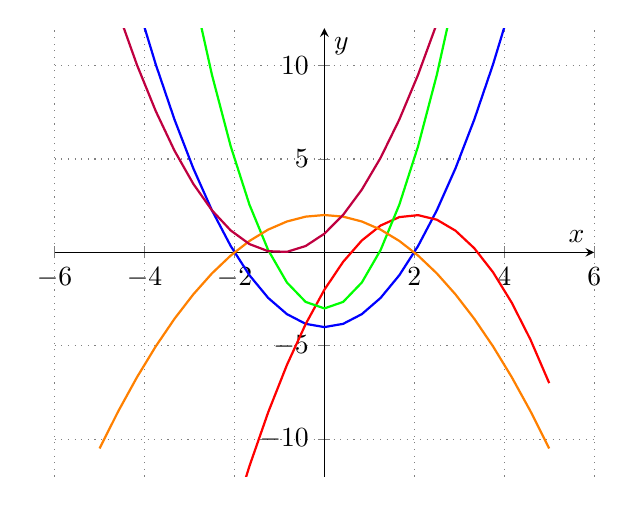
\begin{tikzpicture}
    \begin{axis}[
        axis lines=middle, % Draw axes at the center
        grid=both, % Enable grid lines
        grid style={dotted, gray}, % Grid line style
        xlabel={$x$}, % Label for x-axis
        ylabel={$y$}, % Label for y-axis
        xmin=-5, xmax=5, % x-axis range
        ymin=-10, ymax=10, % y-axis range
        enlargelimits=true, % Allow some space around plots
        legend pos=north west, % Position of the legend
        legend style={font=\small} % Style of legend text
    ]

    % Plot the first quadratic
    \addplot[thick, blue] {x^2 - 4};

    % Plot the second quadratic
    \addplot[thick, red] {-x^2 + 4*x - 2};

    % Plot the third quadratic
    \addplot[thick, green] {2*x^2 - 3};

    % Plot the fourth quadratic
    \addplot[thick, orange] {-0.5*x^2 + 2};

    % Plot the fifth quadratic
    \addplot[thick, purple] {x^2 + 2*x + 1};

    \end{axis}
\end{tikzpicture}

\end{document}
